\documentclass[tikz,border=10pt]{standalone}
\usepackage[T1]{fontenc}
\usepackage{lmodern}
\usepackage{tikz}
\usetikzlibrary{arrows.meta,calc,decorations.pathreplacing,fit,matrix,positioning}

\definecolor{cornellred}{HTML}{B31B1B}
\definecolor{ink}{HTML}{202124}
\definecolor{muted}{HTML}{667085}
\definecolor{line}{HTML}{AEB8C6}
\definecolor{paper}{HTML}{FFFFFF}
\definecolor{soft}{HTML}{F5F7FA}
\definecolor{camera}{HTML}{E8F4FF}
\definecolor{memory}{HTML}{F0F7EC}
\definecolor{compute}{HTML}{FFF3E6}
\definecolor{display}{HTML}{F7ECF3}
\definecolor{verify}{HTML}{EFEAFE}

\tikzset{
  font=\sffamily,
  flow/.style={
    -{Latex[length=2.6mm,width=1.8mm]},
    draw=muted,
    line width=0.8pt,
    rounded corners=2pt
  },
  dataflow/.style={
    flow,
    draw=cornellred
  },
  block/.style={
    rectangle,
    rounded corners=3pt,
    draw=line,
    line width=0.8pt,
    fill=paper,
    align=center,
    minimum width=28mm,
    minimum height=10mm,
    inner xsep=4pt,
    inner ysep=4pt
  },
  smallblock/.style={
    block,
    minimum width=22mm,
    minimum height=8mm,
    font=\sffamily\scriptsize
  },
  title/.style={
    font=\sffamily\bfseries\large,
    text=ink
  },
  labeltext/.style={
    font=\sffamily\scriptsize,
    text=muted,
    align=center
  },
  camera_block/.style={block, fill=camera, draw=blue!45!black},
  memory_block/.style={block, fill=memory, draw=green!45!black},
  compute_block/.style={block, fill=compute, draw=orange!65!black},
  display_block/.style={block, fill=display, draw=purple!45!black},
  verify_block/.style={block, fill=verify, draw=violet!50!black},
  groupbox/.style={
    draw=line,
    rounded corners=5pt,
    line width=0.7pt,
    fill=soft,
    inner sep=7pt
  }
}


% Put groupbox backdrops on a dedicated background layer so they
% don't paint over the compute_blocks they enclose.
\pgfdeclarelayer{background}
\pgfsetlayers{background,main}

\begin{document}
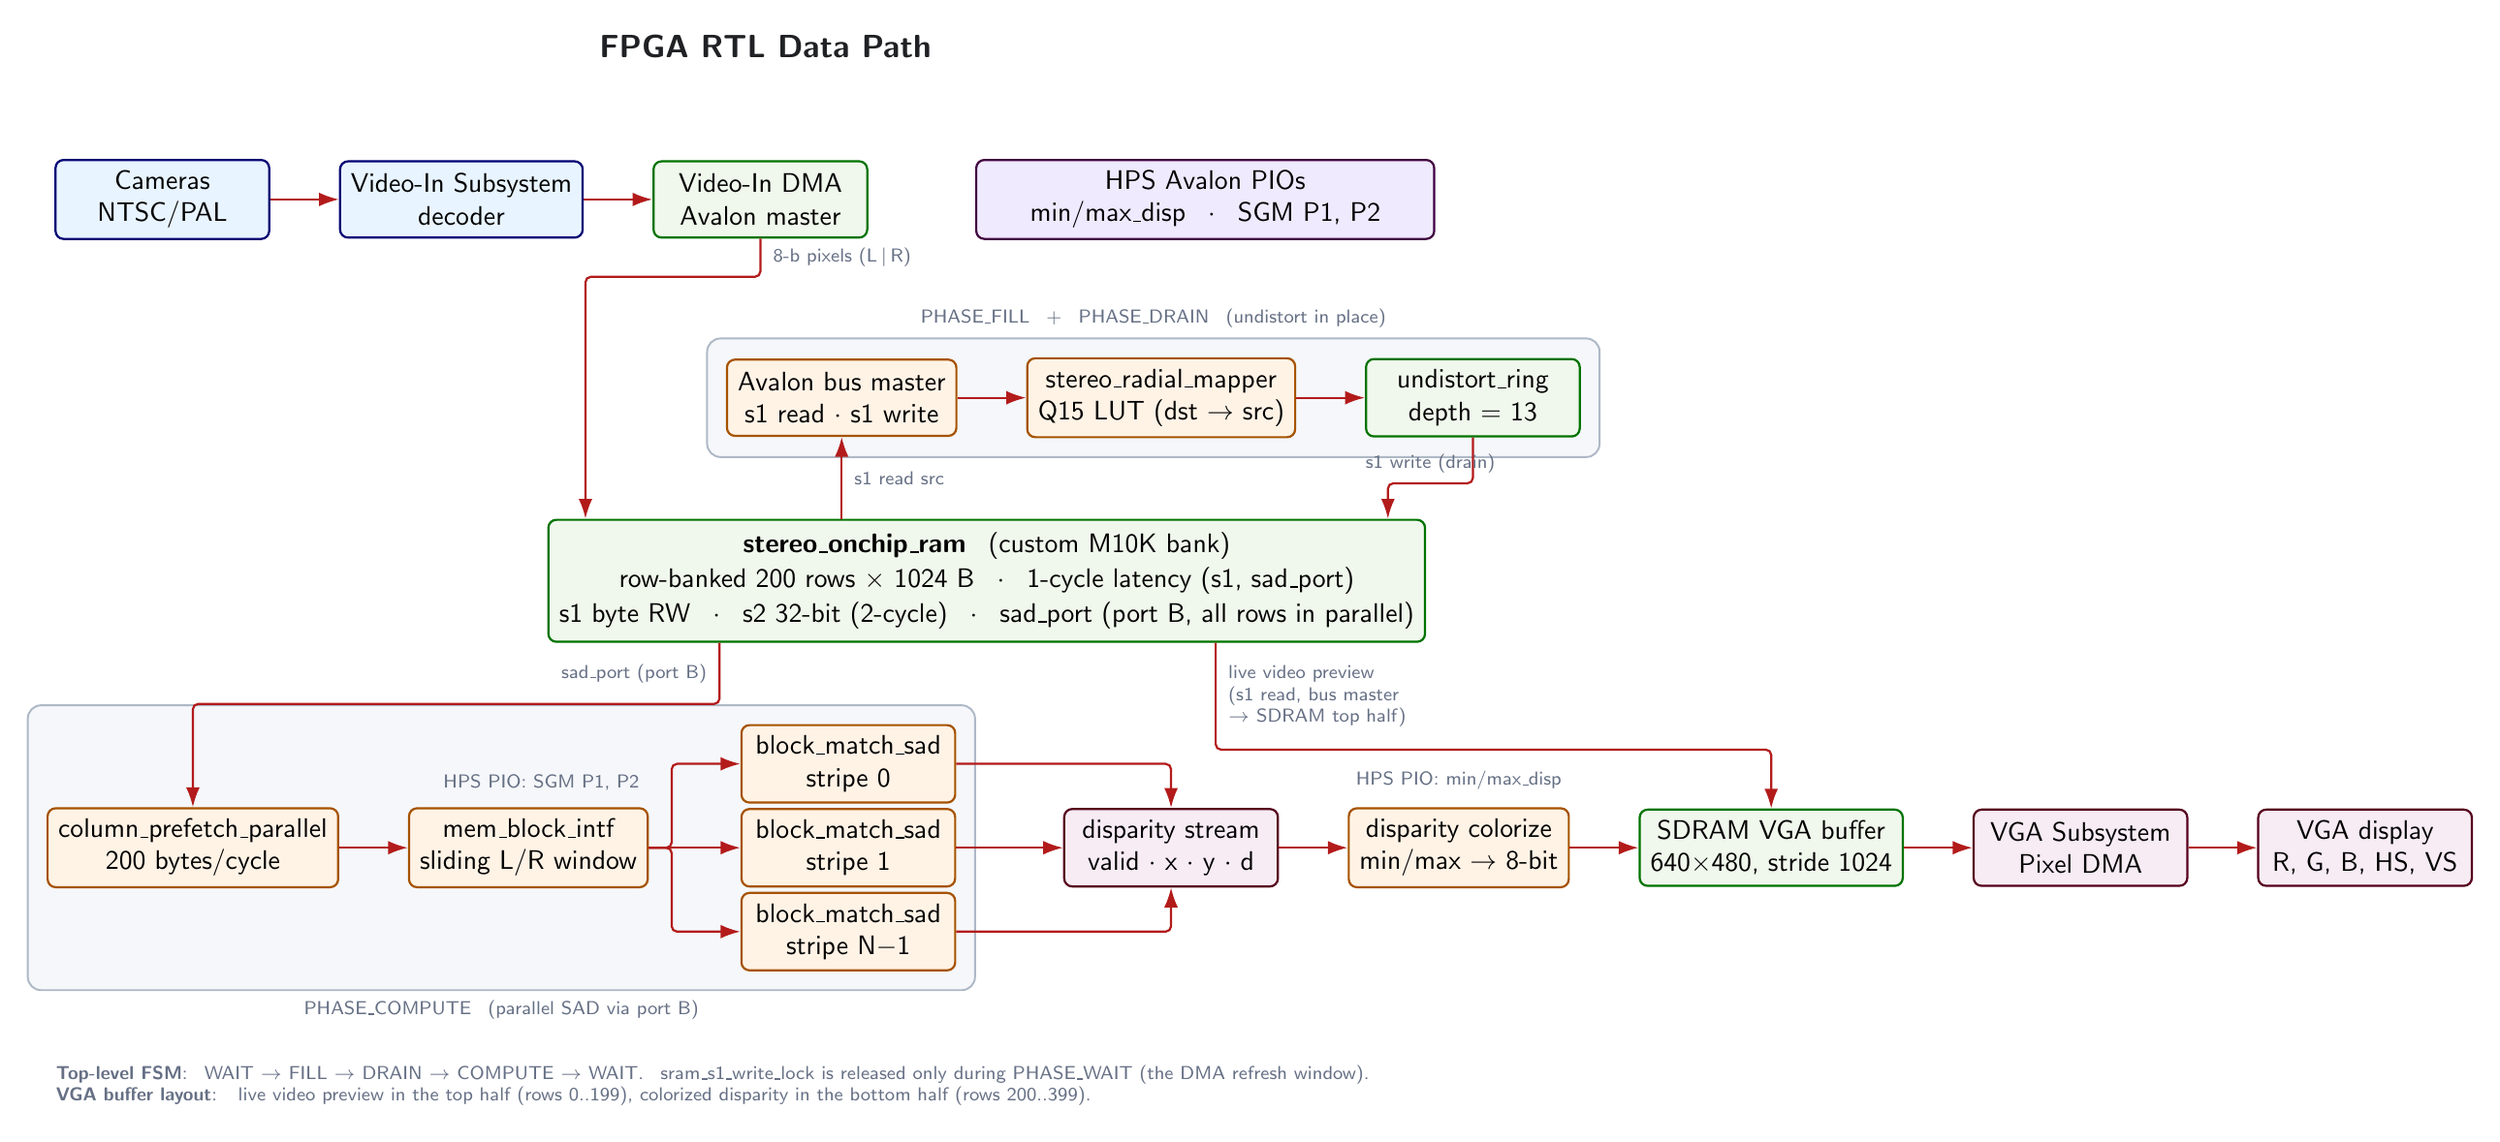
\begin{tikzpicture}[node distance=7mm and 9mm]

  \node[title] at (-1.5, 7.6) {FPGA RTL Data Path};

  %====================================================================
  % Capture chain (top-left)
  %====================================================================
  \node[camera_block]                 (cams)  at (-9.4, 5.6) {Cameras\\NTSC/PAL};
  \node[camera_block, right=of cams]  (dec)                  {Video-In Subsystem\\decoder};
  \node[memory_block, right=of dec]   (vdma)                 {Video-In DMA\\Avalon master};

  %====================================================================
  % HPS Avalon PIOs (top-right)
  %====================================================================
  \node[verify_block, right=14mm of vdma, minimum width=60mm] (hps)
    {HPS Avalon PIOs\\
     min/max\_disp \, $\cdot$ \, SGM P1, P2};

  %====================================================================
  % Rectification loop (FILL + DRAIN phases) — placed above the SRAM
  % and clearly to the right of the vdma → SRAM descent so the
  % capture arrow does not pass through this groupbox.
  %====================================================================
  \node[compute_block] (busio) at (-0.5, 3.0)
    {Avalon bus master\\s1 read $\cdot$ s1 write};
  \node[compute_block, right=of busio] (mapper)
    {stereo\_radial\_mapper\\Q15 LUT (dst $\to$ src)};
  \node[memory_block, right=of mapper] (ring)
    {undistort\_ring\\depth = 13};

  %====================================================================
  % Central SRAM hub
  %====================================================================
  \node[memory_block, minimum width=90mm, minimum height=16mm] (sram) at (1.4, 0.6)
    {\textbf{stereo\_onchip\_ram} \, (custom M10K bank)\\[1pt]
     row-banked 200 rows $\times$ 1024 B \, $\cdot$ \, 1-cycle latency (s1, sad\_port)\\[1pt]
     s1 byte RW \, $\cdot$ \, s2 32-bit (2-cycle) \, $\cdot$ \, sad\_port (port B, all rows in parallel)};

  %====================================================================
  % SAD compute pipeline (below SRAM) — PHASE_COMPUTE
  %====================================================================
  \node[compute_block] (cpref) at (-9.0, -2.9)
    {column\_prefetch\_parallel\\200 bytes/cycle};
  \node[compute_block, right=of cpref] (mbi)
    {mem\_block\_intf\\sliding L/R window};

  \node[compute_block, right=12mm of mbi, yshift= 11mm] (sad0)
    {block\_match\_sad\\stripe 0};
  \node[compute_block, right=12mm of mbi]               (sad1)
    {block\_match\_sad\\stripe 1};
  \node[compute_block, right=12mm of mbi, yshift=-11mm] (sadN)
    {block\_match\_sad\\stripe N$-$1};

  \node[display_block, right=14mm of sad1] (disp)
    {disparity stream\\valid $\cdot$ x $\cdot$ y $\cdot$ d};

  %====================================================================
  % Output chain — same row as disp so the disp → color arrow is a
  % short, clean horizontal hop instead of a long L-bend across the
  % SAD groupbox.
  %====================================================================
  \node[compute_block, right=of disp]    (color)  {disparity colorize\\min/max $\to$ 8-bit};
  \node[memory_block,  right=of color]   (vbuf)   {SDRAM VGA buffer\\640$\times$480, stride 1024};
  \node[display_block, right=of vbuf]    (vgasub) {VGA Subsystem\\Pixel DMA};
  \node[display_block, right=of vgasub]  (vga)    {VGA display\\R, G, B, HS, VS};

  %====================================================================
  % HPS PIO usage cues
  %====================================================================
  \node[labeltext, anchor=south east, font=\sffamily\scriptsize, text=muted, align=right]
     at ($(mbi.north east) + (0,1mm)$) {HPS PIO: SGM P1, P2};
  \node[labeltext, anchor=south, font=\sffamily\scriptsize, text=muted, align=center]
     at ($(color.north) + (0,1mm)$) {HPS PIO: min/max\_disp};

  %====================================================================
  % Arrows — capture chain into SRAM
  %====================================================================
  \draw[dataflow] (cams) -- (dec);
  \draw[dataflow] (dec)  -- (vdma);
  \draw[dataflow] (vdma.south) -- ++(0,-5mm)
     node[labeltext, midway, right=1pt]{8-b pixels (L\,$|$\,R)}
     -| ($(sram.north west) + (5mm,0)$);

  %====================================================================
  % Rectification loop: SRAM → busio → mapper → ring → SRAM. With the
  % group above SRAM, the read-src arrow is a straight vertical at
  % busio's x, and the write-drain arrow drops out of ring, jogs left
  % across the gap between groupbox bottom and SRAM top, and dives in.
  %====================================================================
  \draw[dataflow] (sram.north -| busio.south) -- (busio.south)
     node[labeltext, midway, right=1pt]{s1 read src};
  \draw[dataflow] (busio) -- (mapper);
  \draw[dataflow] (mapper) -- (ring);
  \draw[dataflow] (ring.south) -- ++(0,-6mm)
     -| node[labeltext, pos=0.25, above]{s1 write (drain)}
     ($(sram.north east) + (-5mm,0)$);

  %====================================================================
  % SAD compute path: SRAM (port B) → cpref → mbi → SAD bank → disp
  %====================================================================
  \draw[dataflow] ($(sram.south) + (-3.5cm,0)$) -- ++(0,-8mm)
     node[labeltext, midway, left=1pt]{sad\_port (port B)}
     -| (cpref.north);
  \draw[dataflow] (cpref) -- (mbi);
  \draw[dataflow] (mbi.east) -- ++(3mm,0) |- (sad0.west);
  \draw[dataflow] (mbi.east) -- (sad1.west);
  \draw[dataflow] (mbi.east) -- ++(3mm,0) |- (sadN.west);

  \draw[dataflow] (sad0.east) -| (disp.north);
  \draw[dataflow] (sad1.east) -- (disp.west);
  \draw[dataflow] (sadN.east) -| (disp.south);

  %====================================================================
  % Disparity stream → colorize → VGA buffer → VGA Subsystem → display
  % (single horizontal flow — no over-the-groupbox routing)
  %====================================================================
  \draw[dataflow] (disp)   -- (color);
  \draw[dataflow] (color)  -- (vbuf);
  \draw[dataflow] (vbuf)   -- (vgasub);
  \draw[dataflow] (vgasub) -- (vga);

  %====================================================================
  % NEW: live video preview path — bus master reads SRAM and writes
  % each pixel to the top half of the SDRAM VGA buffer during FILL.
  % Routed to the right of the SAD groupbox so it doesn't tangle.
  %====================================================================
  \draw[dataflow] ($(sram.south) + (3.0cm,0)$) -- ++(0,-1.4cm)
     node[labeltext, midway, right=1pt, align=left]
        {live video preview\\(s1 read, bus master\\$\to$ SDRAM top half)}
     -| (vbuf.north);

  %====================================================================
  % Group annotations (FSM phases) — on background layer
  %====================================================================
  \begin{pgfonlayer}{background}
    \node[groupbox, fit=(busio)(mapper)(ring),
          label={[labeltext]above:PHASE\_FILL \, + \, PHASE\_DRAIN \, (undistort in place)}] {};
    \node[groupbox, fit=(cpref)(mbi)(sad0)(sad1)(sadN),
          label={[labeltext]below:PHASE\_COMPUTE \, (parallel SAD via port B)}] {};
  \end{pgfonlayer}

  %====================================================================
  % Footer: FSM order + write-lock note. Placed well below the
  % PHASE_COMPUTE groupbox label so the two don't collide.
  %====================================================================
  \node[labeltext, align=left, anchor=north west]
     at ($(cpref.south west) + (0mm,-22mm)$)
     {\textbf{Top-level FSM}: \,
      WAIT $\to$ FILL $\to$ DRAIN $\to$ COMPUTE $\to$ WAIT.
      \, sram\_s1\_write\_lock is released only during PHASE\_WAIT (the DMA refresh window).\\
      \textbf{VGA buffer layout}: \,
      live video preview in the top half (rows 0..199), colorized disparity in the bottom half (rows 200..399).};

\end{tikzpicture}
\end{document}
